\documentclass[12pt, letterpaper]{article}

\usepackage[utf8]{inputenc}
\usepackage{hyperref}
\usepackage{epsfig, url}
\usepackage{epstopdf}
\usepackage{graphicx}
\usepackage{datetime}
\usepackage{multirow}
\usepackage{rotating}


%\usepackage{wrapfig}
%\usepackage{amsmath}
\usepackage{amssymb}
\usepackage{geometry} 
\geometry{a4paper}              

\usepackage{titling}

\setlength{\evensidemargin}{0in}
\setlength{\oddsidemargin}{0in}
\setlength{\textwidth}{6.5in}
\setlength{\textheight}{9.0in}
\setlength{\topmargin}{0in}
\setlength{\headheight}{0in}
\setlength{\headsep}{0in}
\setlength{\itemsep}{-\parsep}



\begin{document}
\title{\large Course CS549 Assignment 1\\[0.5cm]
        \bf\Large Implementation of the DES algorithm}
\author{\large Sreeparna Das (226101004)\\
\\
        \large Vishal Kumar (226101005)\\
\\
        \large Akash Lal Dutta (226101001)}
        
\date{February 19, 2023}
\makeatletter
    \begin{titlepage}
        \begin{center}
        \vbox{}\vspace{5cm}
            {\@title }\\[3cm] 
            {\@author}\\
            %{Instructor: \bf instructor name}\\
            \vfill 
\includegraphics[scale=0.2]{images/IITG_logo.png}\\[0.4cm]
            {\@date}
        \end{center}
    \end{titlepage}
\makeatother
%\thispagestyle{empty}




\newpage
\tableofcontents
\newpage
\listoftables
\listoffigures
\newpage

\addcontentsline{toc}{section}{\nameref{intro}}
\section*{The DES Algorithm : Introduction}
\label{intro}
The Data Encryption Standard (DES) algorithm is a symmetric-key block cipher used for encrypting and decrypting digital data. It takes a 64-bit block of plain-text and a 64-bit key as inputs, and produces a 64-bit block of cipher-text as output.\\
\\
The algorithm consists of 16 rounds, each using a different 48-bit sub-key generated from the original 64-bit key. In each round, the 64-bit plain-text is first split into two 32-bit halves, and then a function is applied to one half using the sub-key. The result is XOR-ed with the other half, and the two halves are swapped before moving on to the next round.\\
\\
The function applied in each round includes an expansion permutation, which expands the 32-bit input into a 48-bit value, and a substitution step, which replaces the 48-bit value with a different 32-bit value using a set of predefined substitution boxes. The output of the substitution step is then subjected to a permutation, known as the P-box permutation, before being XOR-ed with the other half.\\
\\
After all 16 rounds have been completed, the final 64-bit output is subjected to a final permutation, which shuffles the bits according to a predetermined pattern to produce the final cipher-text.\\
\\
The same algorithm and key are used for encryption and decryption, the only difference being the order in which the sub-keys are used in the rounds.


\section{Structure of a key in DES Algorithm}
\label{Hand-cal}
The key in the DES algorithm is a 64-bit value used to encrypt and decrypt data. The key undergoes transformation and permutation during the key generation process to create 16 sub-keys, one for each of the 16 rounds of the DES algorithm. Each sub-key is a 48-bit value used to modify the plain-text during each round of encryption or decryption. The sub-keys are generated from the original 64-bit key through permutation, shifting, and compression.\\
\\
The DES algorithm uses a technique known as the Feistel network, which means that the data is divided into two halves, left and right, and each half undergoes a series of modifications using the sub-keys. The left and right halves are swapped after each round, and the modifications are repeated. The sub-keys are generated using a combination of the original key and the results of the previous round of modifications.\\
\\
The key plays a crucial role in the DES algorithm, as it determines the encryption and decryption process. To ensure the security of the data, it is important to choose a strong and unique key. However, the DES algorithm has since been replaced by more secure encryption algorithms such as AES.

\begin{figure}[hbt!]
    \centering
    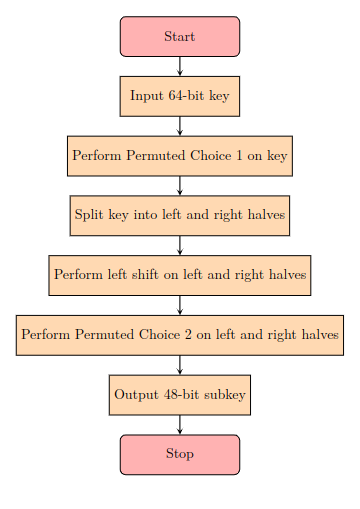
\includegraphics[scale=0.6, angle=0]{images/Screenshot from 2023-02-18 21-07-04.png}
    \caption{Flowchart of the Key Generation}
    \label{fig:crazy}
\end{figure}


\section{Implementation of DES Algorithm}

\begin{enumerate}
\item \textbf{Key Generation:} The 64-bit key can be input as a string of hexadecimal characters and converted to a binary string. The key generation algorithm can then be implemented to produce 16 round sub-keys of 48-bits each.

\item \textbf{Initial Permutation:} The 64-bit plain-text can also be input as a string of hexadecimal characters and converted to a binary string. The initial permutation algorithm can then be implemented to rearrange the bits according to a fixed permutation table.

\item \textbf{Round Function:} The 64-bit plain-text can be divided into 32-bit blocks (LPT and RPT) using slicing. Each round can then consist of the following steps:

\begin{enumerate}
\item Expansion Permutation: The RPT block can be expanded from 32-bits to 48-bits using a fixed permutation table.

\item Subkey Mixing: The expanded RPT block can be XORed with the corresponding 48-bit subkey for that round. The subkeys can be generated by selecting the appropriate 48-bits from the round subkeys produced in the key generation step.

\item S-Box Substitution: The resulting 48-bit block can then be divided into 8 6-bit blocks, each of which is substituted using a fixed S-box. The S-boxes can be implemented using lookup tables.

\item Permutation: The resulting 32-bit block can be rearranged using a fixed permutation table.

\item LPT and RPT Update: The resulting 32-bit block can be XORed with the LPT block, and the RPT block becomes the new LPT block.
\end{enumerate}

\item \textbf{Final Permutation:} After the 16 rounds are completed, the LPT and RPT can be swapped and then subjected to a final permutation using a fixed permutation table to produce the 64-bit ciphertext.
\end{enumerate}
The output of each step in the DES algorithm, including the LPT and RPT after each round and the ciphertext, can be printed or stored in variables for further analysis.

\begin{figure}[hbt!]
    \centering
    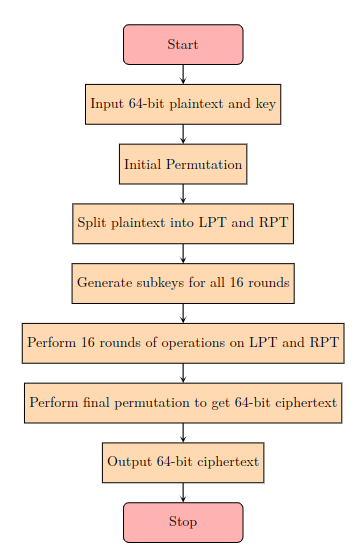
\includegraphics[scale=0.6, angle=0]{images/Screenshot from 2023-02-18 21-05-04.png}
    \caption{DES Algorithm}
    \label{fig:crazy}
\end{figure}



        
\section{Assignment Overview}

In our case, the 64-bit plain-text is formed using the last eight digits of two students' roll numbers, and the 64-bit key is formed using the last eight digits of two other students' roll numbers. The output of each step in the DES algorithm, including the \textbf{LPT} and \textbf{RPT} after each round and the cipher-text, should be documented for the given input.

    \subsection{Results to be produced}

    \begin{enumerate}
  \item Initial permutation (mention LPT and RPT)
  \item For all 16 rounds:
  \begin{enumerate}
    \item Expansion permutation
    \item Sub-key used in the round
    \item LPT and RPT after the round
  \end{enumerate}
  \item Final permutation (mention Cipher-text)
\end{enumerate}

\subsection{Given Data}

\begin{table}[h]
    \centering
    \begin{tabular}{|c|c|}
        \hline
        \textbf{Student Name} & \textbf{Roll Number} \\
        \hline
        Sreeparna Das & 26101004 \\
        \hline
        Vishal Kumar & 26101005 \\
        \hline
        Akash Lal Dutta & 26101001 \\
        \hline
        Dummy Name & 26101006 \\
        \hline
    \end{tabular}
    \caption{Student Information}
    \label{tab:student-info}
\end{table} \\



\subsection{{For student S1 :}}

\begin{table}[h]
    \centering
    \begin{tabular}{|c|c|}
        \hline
          Plain Text & Key \\
        \hline
        \textbf{S1 S2} & \textbf{S3 S4} \\
        \hline
    \end{tabular}
    \caption{Plain-Text and Key for S1}
    \label{tab:text-key}
\end{table}






\underline{\textbf{Initial Permutation}} \\
\\
\begin{table}[h]
    \centering
    \begin{tabular}{|c|c|}
        
        \hline
        LPT & RPT \\
        \hline
        00669980 & 00110011   \\
        \hline
    \end{tabular}
    \caption{LPT and RPT Values}
    \label{tab:lpt-rpt}
\end{table}

\begin{table}[h]
    \centering
    \begin{tabular}{|c|c|}
        
        \hline
        Round & Exapansion Permutation \\
        \hline
        1 & 8000A28000A2   \\
        \hline
        2 & AAA95C2080FA
        \\
        \hline
        3  & 9595000A7D06
        \\
         \hline
        4 & 40D550258251
        \\
         \hline
        5 & 3A68FBDAAAA0
        \\
         \hline
        6 & 7F4302850051
        \\
         \hline
        7 & 9AAAF830565E
        \\
         \hline
        8 & 156BF80F95AC
        \\
         \hline
        9 & 95C15970965A
        \\
         \hline
        10 & 504252BAC005
        \\
         \hline
        11 & E041A82FD553
        \\
         \hline
        12 & 10EB0AB07C54
        \\
         \hline
        13 & 2FA90D7517FC
        \\
         \hline
        14 & 1F3F01600004
        \\
         \hline
        15 & 8AE8AC25D702
        \\
         \hline
        16 & 6F7FAFE01609
        \\
        \hline
        
    \end{tabular}
    \caption{Expansion Permutation}
    \label{tab:lpt-rpt}
\end{table}

\begin{table}[ht]
  \centering
  
  \label{tab:sample-table}
    \begin{tabular}{|c|c|c|}
    
      \hline
    Round & LPT & RPT  \\
    \hline
    1 & 00110011 & 552E441D  \\
        \hline
    2 & 552E441D & 2CA013A3

  \\
         \hline
    3 & 2CA013A3 & 86A84C48  \\
         \hline
    4 & 86A84C48 & 731DB550   \\
         \hline
    5 & 731DB550 & FA610808  \\
        \hline
    6 & FA610808 & 355C62CF   \\
         \hline
    7 &  355C62CF & 2B7C1CB6

  \\
         \hline
    8 & 2B7C1CB6 & 2E2CE4CD

 

  \\
         \hline
    9 & 2E2CE4CD

 & A2497602

  \\
         \hline
    10 & A2497602

 & C2345EA9

  \\
         \hline
    11 & C2345EA9

 & 2765638A

  \\
         \hline
    12 & 2765638A

 & 5D26E8FE

  \\
         \hline
    13 & 5D26E8FE

 & 39E0C002 \\
         \hline
    14 & 39E0C002 & 17164EE1

  \\
         \hline
    15 & 17164EE1

 & DBF7C0C4

  \\
         \hline
    16 & DBF7C0C4

 & B7FB57BD

  \\
    \hline
  \end{tabular}
    \caption{LPT and RPT values after each of 16 Rounds}

    

\end{table}





\begin{table}[h]
    \centering
    \begin{tabular}{|c|c|}
        \hline
        \textbf{Round} & \textbf{Sub-Key} \\
        \hline
        1 & 000C80200344
 \\
        \hline
        2 & 1000004600D0
 \\
        \hline
        3 & 00082401A14D
 \\
        \hline
        4 & 802004229480
 \\
        \hline
        5 & 000620480527
 \\
        \hline 
        6 & C010200E4888
 \\
        \hline
        7 & 808240405151
 \\
        \hline
        8 & 005202838028
 \\
        \hline
        9 & 24020001465A
 \\
        \hline
        10 & 0210101D9000
 \\
        \hline
        11 & 0C0050804464
 \\
        \hline
        12 & 06400808AA84 \\
        \hline
        13 & 0A0100B04491 \\
        \hline
        14 & 0808090B0203
 \\
        \hline
        15 & 012008966100 \\
        \hline
        16 & 10008C150807 \\
        \hline

    \end{tabular}
    \caption{Sub-Key values after each of 16 rounds}
    \label{tab:student-info}
\end{table}



\begin{table}[h]
    \centering
    \begin{tabular}{|c|}
        \hline
          Cipher Text \\
        \hline
           FAF89B62FAB27DF7
  \\
        \hline
    \end{tabular}
    \caption{Cipher Text Generated}
    \label{tab:text-key}
\end{table}

\clearpage

\subsection{{For student S2 :}}

\begin{table}[h]
    \centering
    \begin{tabular}{|c|c|}
        \hline
          Plain Text & Key \\
        \hline
        \textbf{S2 S3} & \textbf{S4 S1} \\
        \hline
    \end{tabular}
    \caption{Plain-Text and Key for S2}
    \label{tab:text-key}
\end{table}






\underline{\textbf{Initial Permutation}} \\
\\
\begin{table}[h]
    \centering
    \begin{tabular}{|c|c|}
        
        \hline
        LPT & RPT \\
        \hline
        00661988 & 00110011   \\
        \hline
    \end{tabular}
    \caption{LPT and RPT Values}
    \label{tab:lpt-rpt}
\end{table}

\begin{table}[h]
    \centering
    \begin{tabular}{|c|c|}
        
        \hline
        Round & Exapansion Permutation \\
        \hline
        1 & 8000A28000A2   \\
        \hline
        2 & A0E95D6000FA
        \\
        \hline
        3  & 0FC2001AFF00
        \\
         \hline
        4 & C0D454306BAF
        \\
         \hline
        5 & F0AA581FBEFF
        \\
         \hline
        6 & B0FD0FDAFFFA
        \\
         \hline
        7 & 7A83540FA905
        \\
         \hline
        8 & 357D0BDA54F8
        \\
         \hline
        9 & 45FD5BF515F9
        \\
         \hline
        10 & A03FA6BA5706
        \\
         \hline
        11 & EF02082F0207
        \\
         \hline
        12 & E595AA9A80FB
        \\
         \hline
        13 & D581FAA043FB
        \\
         \hline
        14 & EF03517A40A3
        \\
         \hline
        15 & 9AFEF680BC5A
        \\
         \hline
        16 & 40D7A7E5D501
        \\
        \hline
        
    \end{tabular}
    \caption{Expansion Permutation}
    \label{tab:lpt-rpt}
\end{table}

\begin{table}[ht]
  \centering
  
  \label{tab:sample-table}
    \begin{tabular}{|c|c|c|}
    
      \hline
    Round & LPT & RPT  \\
    \hline
    1 & 00110011 & 472EC01D  \\
        \hline
    2 & 472EC01D & 1E4037E0

  \\
         \hline
    3 & 1E4037E0 & 868A6377  \\
         \hline
    4 & 868A6377 & E54C3DDF   \\
         \hline
    5 & E54C3DDF & 67A7B7FD  \\
        \hline
    6 & 67A7B7FD & F46A1D22   \\
         \hline
    7 &  F46A1D22 & 6BA5B29C

  \\
         \hline
    8 & 6BA5B29C & 8FADE8BC

 

  \\
         \hline
    9 & 8FADE8BC

 & 41F372E3

  \\
         \hline
    10 & 41F372E3

 & D8445843

  \\
         \hline
    11 & D8445843

 & CCB5341D

  \\
         \hline
    12 & CCB5341D

 & AC3D427D

  \\
         \hline
    13 & AC3D427D

 & D868F211 \\
         \hline
    14 & D868F211 & 37DB058D

  \\
         \hline
    15 & 37DB058D

 & 86F3CEA0

  \\
         \hline
    16 & 86F3CEA0

 & 9EC7A381

  \\
    \hline
  \end{tabular}
    \caption{LPT and RPT values after each of 16 Rounds}

    

\end{table}





\begin{table}[h]
    \centering
    \begin{tabular}{|c|c|}
        \hline
        \textbf{Round} & \textbf{Sub-Key} \\
        \hline
        1 & 000C80210241
 \\
        \hline
        2 & 1000006202D0
 \\
        \hline
        3 & 00082411810F
 \\
        \hline
        4 & 802004061480
 \\
        \hline
        5 & 000620482165
 \\
        \hline 
        6 & C0102022C888
 \\
        \hline
        7 & 808240401513
 \\
        \hline
        8 & 0052028F0028
 \\
        \hline
        9 & 240200014662
 \\
        \hline
        10 & 0210105C8800
 \\
        \hline
        11 & 0C005080445C
 \\
        \hline
        12 & 06400809B280 \\
        \hline
        13 & 0A0100B04421 \\
        \hline
        14 & 0808090A0A06
 \\
        \hline
        15 & 012008946190 \\
        \hline
        16 & 10008C852805 \\
        \hline

    \end{tabular}
    \caption{Sub-Key values after each of 16 rounds}
    \label{tab:student-info}
\end{table}



\begin{table}[h]
    \centering
    \begin{tabular}{|c|}
        \hline
          Cipher Text \\
        \hline
           3AFCE484901934FF
  \\
        \hline
    \end{tabular}
    \caption{Cipher Text Generated}
    \label{tab:text-key}
\end{table}

\clearpage










\subsection{{For student S3 :}}

\begin{table}[h]
    \centering
    \begin{tabular}{|c|c|}
        \hline
          Plain Text & Key \\
        \hline
        \textbf{S3 S4} & \textbf{S2 S1} \\
        \hline
    \end{tabular}
    \caption{Plain-Text and Key for S3}
    \label{tab:text-key}
\end{table}






\underline{\textbf{Initial Permutation}} \\
\\
\begin{table}[h]
    \centering
    \begin{tabular}{|c|c|}
        
        \hline
        LPT & RPT \\
        \hline
        00669108 & 00110091   \\
        \hline
    \end{tabular}
    \caption{LPT and RPT Values}
    \label{tab:lpt-rpt}
\end{table}

\begin{table}[h]
    \centering
    \begin{tabular}{|c|c|}
        
        \hline
        Round & Exapansion Permutation \\
        \hline
        1 & 8000A28014A2   \\
        \hline
        2 & A0E8FC2594AA
        \\
        \hline
        3  & 9001A685EA5A
        \\
         \hline
        4 & 4F55A14A7E09
        \\
         \hline
        5 & 9FD4F0152AA6
        \\
         \hline
        6 & AF7D53CFAAAA
        \\
         \hline
        7 & 209557CA9608
        \\
         \hline
        8 & 0A6856A5BDA4
        \\
         \hline
        9 & B594081F8002
        \\
         \hline
        10 & 20D45BE5545C
        \\
         \hline
        11 & 70BEF82543F9
        \\
         \hline
        12 & 10805FEF7F54
        \\
         \hline
        13 & FA170FDA3D5F
        \\
         \hline
        14 & FA42FA8F570B
        \\
         \hline
        15 & CFBFAAB081AB
        \\
         \hline
        16 & 5094F0209605
        \\
        \hline
        
    \end{tabular}
    \caption{Expansion Permutation}
    \label{tab:lpt-rpt}
\end{table}

\begin{table}[ht]
  \centering
  
  \label{tab:sample-table}
    \begin{tabular}{|c|c|c|}
    
      \hline
    Round & LPT & RPT  \\
    \hline
    1 & 00110091 & 471E4C95  \\
        \hline
    2 & 471E4C95 & 20330F4D

  \\
         \hline
    3 & 20330F4D & 9AB093C4  \\
         \hline
    4 & 9AB093C4 & 3E982953   \\
         \hline
    5 & 3E982953 & 5BA99D55  \\
        \hline
    6 & 5BA99D55 & 44AB94C4   \\
         \hline
    7 &  44AB94C4 & 130B4DB2

  \\
         \hline
    8 & 130B4DB2 & 6C843C01

 

  \\
         \hline
    9 & 6C843C01

 & 468DCA8E

  \\
         \hline
    10 & 468DCA8E

 & E5DC4A7C

  \\
         \hline
    11 & E5DC4A7C

 & 240FDBEA

  \\
         \hline
    12 & 240FDBEA

 & F0E7B1AF

  \\
         \hline
    13 & F0E7B1AF

 & F25D1AE5 \\
         \hline
    14 & F25D1AE5 & 9DF56435

  \\
         \hline
    15 & 9DF56435

 & A49844C2

  \\
         \hline
    16 & A49844C2

 & D5FD2EC3

  \\
    \hline
  \end{tabular}
    \caption{LPT and RPT values after each of 16 Rounds}

    

\end{table}





\begin{table}[h]
    \centering
    \begin{tabular}{|c|c|}
        \hline
        \textbf{Round} & \textbf{Sub-Key} \\
        \hline
        1 & 000C80210244
 \\
        \hline
        2 & 1000004202D0
 \\
        \hline
        3 & 00082411A10D                                                                  
 \\
        \hline
        4 & 802004229480
 \\
        \hline
        5 & 000620482127
 \\
        \hline 
        6 & C01020264888
 \\
        \hline
        7 & 808240401153
 \\
        \hline
        8 & 005202878028
 \\
        \hline
        9 & 24020001464A
 \\
        \hline
        10 & 0210105C9000
 \\
        \hline
        11 & 0C005080446C
 \\
        \hline
        12 & 06400808BA80 \\
        \hline
        13 & 0A0100B04431 \\
        \hline
        14 & 0808090B0A02
 \\
        \hline
        15 & 012008946110 \\
        \hline
        16 & 10008C950805 \\
        \hline

    \end{tabular}
    \caption{Sub-Key values after each of 16 rounds}
    \label{tab:student-info}
\end{table}



\begin{table}[h]
    \centering
    \begin{tabular}{|c|}
        \hline
          Cipher Text \\
        \hline
           A20BEC38B068A7F3
  \\
        \hline
    \end{tabular}
    \caption{Cipher Text Generated}
    \label{tab:text-key}
\end{table}

\clearpage


\subsection{{For student S4 :}}

\begin{table}[h]
    \centering
    \begin{tabular}{|c|c|}
        \hline
          Plain Text & Key \\
        \hline
        \textbf{S4 S1} & \textbf{S3 S2} \\
        \hline
    \end{tabular}
    \caption{Plain-Text and Key for S4}
    \label{tab:text-key}
\end{table}






\underline{\textbf{Initial Permutation}} \\
\\
\begin{table}[h]
    \centering
    \begin{tabular}{|c|c|}
        
        \hline
        LPT & RPT \\
        \hline
        00669900 & 00110019   \\
        \hline
    \end{tabular}
    \caption{LPT and RPT Values}
    \label{tab:lpt-rpt}
\end{table}

\begin{table}[h]
    \centering
    \begin{tabular}{|c|c|}
        
        \hline
        Round & Exapansion Permutation \\
        \hline
        1 & 8000A28000F2   \\
        \hline
        2 & 2FA95C2015F8
        \\
        \hline
        3  & 35E8A82F28A4
        \\
         \hline
        4 & DFFCA56002FF
        \\
         \hline
        5 & 5056FC2AE851
        \\
         \hline
        6 & 4A150EBF4355
        \\
         \hline
        7 & 153E5EA54254
        \\
         \hline
        8 & 85AB5E807C0E
        \\
         \hline
        9 & 9FAA5D5ABEA2
        \\
         \hline
        10 & 3A5556BFAA58
        \\
         \hline
        11 & D5550FDFABF3
        \\
         \hline
        12 & 7FFC515A7C0D
        \\
         \hline
        13 & 0F54582A7EA4
        \\
         \hline
        14 & 2A1753EFEA0C
        \\
         \hline
        15 & 053C0805280C
        \\
         \hline
        16 & DFD457D04207
        \\
        \hline
        
    \end{tabular}
    \caption{Expansion Permutation}
    \label{tab:lpt-rpt}
\end{table}

\begin{table}[ht]
  \centering
  
  \label{tab:sample-table}
    \begin{tabular}{|c|c|c|}
    
      \hline
    Round & LPT & RPT  \\
    \hline
    1 & 00110019 & 5D2E40BC  \\
        \hline
    2 & 5D2E40BC & 6F145912

  \\
         \hline
    3 & 6F145912 & BF92C05F  \\
         \hline
    4 & BF92C05F & A2DE5708   \\
         \hline
    5 & A2DE5708 & 90A77A6A  \\
        \hline
    6 & 90A77A6A & 29CF4A4A   \\
         \hline
    7 &  29CF4A4A & 0D6F0387

  \\
         \hline
    8 & 0D6F0387 & 3D4EB5D1

 

  \\
         \hline
    9 & 3D4EB5D1

 & 72AB7D4C

  \\
         \hline
    10 & 72AB7D4C

 & AAA7BD79

  \\
         \hline
    11 & AAA7BD79

 & FF88B386

  \\
         \hline
    12 & FF88B386

 & 1A8C53D2

  \\
         \hline
    13 & 1A8C53D2

 & 50E9DF46 \\
         \hline
    14 & 50E9DF46 & 09840906

  \\
         \hline
    15 & 09840906

 & BE8BA243

  \\
         \hline
    16 & BE8BA243

 & 497A2AD5

  \\
    \hline
  \end{tabular}
    \caption{LPT and RPT values after each of 16 Rounds}

    

\end{table}





\begin{table}[h]
    \centering
    \begin{tabular}{|c|c|}
        \hline
        \textbf{Round} & \textbf{Sub-Key} \\
        \hline
        1 & 000C80200244
 \\
        \hline
        2 & 1000004200D0
 \\
        \hline
        3 & 00082401A10D                                                                  
 \\
        \hline
        4 & 802004221480
 \\
        \hline
        5 & 000620480127
 \\
        \hline 
        6 & C01020064888
 \\
        \hline
        7 & 808240401151
 \\
        \hline
        8 & 005202838028
 \\
        \hline
        9 & 24020001464A
 \\
        \hline
        10 & 0210101C9000
 \\
        \hline
        11 & 0C0050804464
 \\
        \hline
        12 & 06400808AA80 \\
        \hline
        13 & 0A0100B04411 \\
        \hline
        14 & 0808090B0202
 \\
        \hline
        15 & 012008946100 \\
        \hline
        16 & 10008C150805 \\
        \hline

    \end{tabular}
    \caption{Sub-Key values after each of 16 rounds}
    \label{tab:student-info}
\end{table}



\begin{table}[h]
    \centering
    \begin{tabular}{|c|}
        \hline
          Cipher Text \\
        \hline
           937D42F8626CA356
  \\
        \hline
    \end{tabular}
    \caption{Cipher Text Generated}
    \label{tab:text-key}
\end{table}

\clearpage





\end{document}










\newpage
\bibliographystyle{ieeetr}
\bibliography{ref}

\end{document}
